\section{Real-data validation: details}\label{app:realdata}

All numbers here are macros generated by \texttt{analysis/real\_numbers.py} from \texttt{experiments/real/results.json}; the pre-registration is \texttt{experiments/real/DESIGN.md} (written before any training or evaluation) and the data provenance \texttt{DATA.md}.

\paragraph{Data.} Panasonic NCR18650PF cell, Kollmeyer, Mendeley Data v1, DOI 10.17632/wykht8y7tg.1, CC BY 4.0 \citep{kollmeyer2018panasonic}; every downloaded file's SHA-256 matches the repository's. Resampled to $dt=1$\,s; input $u$ = mean current over the second (discharge positive); outputs $y=(\Delta T, V_m)$: case-temperature rise and the terminal voltage behind the plant's 2-s acquisition filter, so that every observer uses the unchanged $y=x[\text{sensors}]$ contract of the simulated battery plant. States $(\mathrm{SOC},V_1,V_2,\Delta T,V_m)$; labelled on real data: SOC (coulomb count), $\Delta T$, $V_m$; $V_1,V_2$ have no labels and are excluded from the phase-2 loss. Split by drive cycle at 25$^\circ$C: train Cycle 1--3, UDDS, LA92; validation Cycle 4; test US06, HWFET (HWFTa and HWFTb pooled), NN; disjoint files and absolute time intervals. Disclosed overlap of shapes: the Cycle 1--4 mixes contain US06/HWFET/NN segments and NN combines US06 and LA92 portions, so the test cycles are new \emph{sequences} on real hardware, not wholly new waveform shapes.

\paragraph{Model identification.} 2-RC equivalent circuit with constant parameters identified by least squares on the training cycles: $R_0=\RealEcmRZero$\,m$\Omega$, $\tau_1=\RealEcmTauOne$\,s, $\tau_2=\RealEcmTauTwo$\,s, $Q=\RealQAh$\,Ah (C/20 capacity), OCV polynomial, lumped thermal model. Open-loop terminal-voltage RMSE \RealVmFitTrainMin--\RealVmFitTrainMax\,mV on the training cycles, \RealVmFitValTestMin--\RealVmFitValTestMax\,mV on validation/test (US06 \RealVmFitUsZeroSix\,mV, errors up to \RealEcmVmax\,V near empty), \RealVmFitZeroMin--\RealVmFitZeroMax\,mV at 0$^\circ$C with Arrhenius-scaled resistances (factor \RealArrheniusFactor): a realistic but incomplete model, as intended.

\paragraph{Observers.} Learned KKL: the paper's default recipe ($n_z=7$, $\alpha=\RealAlpha$/min so that $dt=1$\,s passes the design gate, SFM context, budget 140k (\RealParamsMin--\RealParamsMax\ parameters per conditioner), 3000 phase-2 steps, \RealNSeeds\ seeds). Phase 1 on the identified circuit (zero-input episodes, collocation states, and the training currents replayed on the model); phase 2 is the unchanged \texttt{train.phase2} on real training windows with the loss restricted to the labelled states. WS-best: per seed, whichever of HyperKKL ($r=4$) and its dense-subspace ablation has the lower validation SOC RMSE (\RealWsChoice); the single-method reading uses the $r=4$ rows (HyperKKL vs EKF: \RealLoraEkfCyclesABetter\ of 3 cycles decided for HyperKKL; vs latent: \RealLoraLatentCyclesABetter\ of 3, differences US06 \RealLoraLatentUSZeroSixDiff\ [\RealLoraLatentUSZeroSixCiLo, \RealLoraLatentUSZeroSixCiHi], HWFET \RealLoraLatentHWFETDiff\ [\RealLoraLatentHWFETCiLo, \RealLoraLatentHWFETCiHi], NN \RealLoraLatentNNDiff\ [\RealLoraLatentNNCiLo, \RealLoraLatentNNCiHi]; per-seed means \RealLoraLatentUSZeroSixSeeds; \RealLoraLatentHWFETSeeds; \RealLoraLatentNNSeeds). Filters: the unchanged EKF/UKF on the identified circuit, $Q,R$ from a 72-point grid scored on the validation cycle with the same wrong-prior protocol (oracle-tuned, as \texttt{ekf\_oracle}); the EKF's chosen $r_{V_m}=\RealEkfRvm$\,V sits at the top of the pre-registered grid (score flat there), the UKF's (\RealUkfRvm\,V) is interior. Reference: coulomb counting from the wrong prior (error 20\% by construction). Episodes: 30-min windows every 5\,min through each discharge (US06 \RealNwinUsZeroSix\ windows, HWFET \RealNwinHwfet, NN \RealNwinNn; validation \RealNwinVal), each run with prior $\mathrm{SOC}_0\pm0.2$ where that stays in $[0,1]$.

\paragraph{Statistics and rules.} Per-window paired differences averaged over prior signs and seeds; 95\% moving-block bootstrap over window start times (block 30\,min, 10\,000 resamples) and per-seed means; a cycle counts only if the CI excludes 0 \emph{and} all seeds agree. H1: WS-best beats the tuned EKF on $\ge2$ of 3 test cycles; H2: WS-best beats latent injection, same rule. Everything else is descriptive.

% generated by analysis/real_numbers.py -- do not edit by hand
\begin{table}[t]
\centering\small
\setlength{\tabcolsep}{5pt}
\caption{Real-data validation: settled SOC RMSE [\% SOC] ($t\ge15$ min of 30-min windows, prior SOC 20\% off) on the three held-out 25$^\circ$C drive cycles and on the validation cycle (Cycle 4, used for model selection and filter tuning only). Learned: mean $\pm$ sd over 3 seeds. WS-best = HyperKKL ($r=4$) or its dense-subspace ablation, whichever has the lower validation RMSE per seed (the pre-registered selection). Same-data baselines (Koopman KF, grey-box EKF/UKF): pending.}
\label{tab:real}
\begin{tabular}{@{}lrrrr@{}}
\toprule
method & US06 & HWFET & NN & validation \\
\midrule
WS-best (HyperKKL $r=4$ or dense ablation, chosen per seed on validation) & \textbf{1.76 $\pm$ 0.15} & \textbf{0.86 $\pm$ 0.05} & \textbf{0.69 $\pm$ 0.04} & 0.71 \\
HyperKKL ($r=4$) & 2.18 $\pm$ 0.59 & 0.91 $\pm$ 0.11 & 0.73 $\pm$ 0.04 & 0.75 \\
dense-subspace ablation & 1.75 $\pm$ 0.25 & 0.93 $\pm$ 0.08 & 0.69 $\pm$ 0.03 & 0.77 \\
latent injection & 2.44 $\pm$ 0.58 & 1.09 $\pm$ 0.10 & 1.25 $\pm$ 0.22 & 1.34 \\
concat (additive) & 7.37 $\pm$ 1.22 & 2.80 $\pm$ 0.14 & 4.51 $\pm$ 0.11 & 4.11 \\
autonomous (no input) & 31.52 $\pm$ 2.65 & 15.54 $\pm$ 0.60 & 31.08 $\pm$ 1.55 & 23.07 \\
EKF (identified 2-RC ECM, $Q,R$ tuned on validation) & 8.85 & 1.19 & 1.95 & 3.25 \\
UKF (same model, tuned) & 9.13 & 1.39 & 1.55 & 3.10 \\
coulomb counting from the wrong prior & 20.00 & 20.00 & 20.00 & 20.00 \\
hyperkkl & 2.18 $\pm$ 0.59 & 0.91 $\pm$ 0.11 & 0.73 $\pm$ 0.04 & 0.75 \\
\bottomrule
\end{tabular}
\end{table}


\paragraph{Results.} H1: learned better on \RealHOneLearnedBetter, EKF better on \RealHOneEkfBetter\ of \RealNTestCycles\ cycles. Paired settled-RMSE differences (WS-best $-$ EKF, \% SOC; CI; per-seed means): US06 \RealWsBestEkfUSZeroSixDiff\ [\RealWsBestEkfUSZeroSixCiLo, \RealWsBestEkfUSZeroSixCiHi] (\RealWsBestEkfUSZeroSixSeeds); HWFET \RealWsBestEkfHWFETDiff\ [\RealWsBestEkfHWFETCiLo, \RealWsBestEkfHWFETCiHi] (\RealWsBestEkfHWFETSeeds); NN \RealWsBestEkfNNDiff\ [\RealWsBestEkfNNCiLo, \RealWsBestEkfNNCiHi] (\RealWsBestEkfNNSeeds). Against the UKF: US06 \RealWsBestUkfUSZeroSixDiff, HWFET \RealWsBestUkfHWFETDiff, NN \RealWsBestUkfNNDiff\ (all CIs below 0, all seeds negative). H2: weight-space better on \RealHTwoWsBetter, latent better on \RealHTwoLatentBetter: US06 \RealWsBestLatentUSZeroSixDiff\ [\RealWsBestLatentUSZeroSixCiLo, \RealWsBestLatentUSZeroSixCiHi] (\RealWsBestLatentUSZeroSixSeeds); HWFET \RealWsBestLatentHWFETDiff\ [\RealWsBestLatentHWFETCiLo, \RealWsBestLatentHWFETCiHi] (\RealWsBestLatentHWFETSeeds); NN \RealWsBestLatentNNDiff\ [\RealWsBestLatentNNCiLo, \RealWsBestLatentNNCiHi] (\RealWsBestLatentNNSeeds). Maximum settled error: US06 WS-best \RealWsBestUSZeroSixMax\,\% vs EKF \RealEkfUSZeroSixMax\,\%; HWFET \RealWsBestHWFETMax\ vs \RealEkfHWFETMax; NN \RealWsBestNNMax\ vs \RealEkfNNMax. Median time to stay within 5\% SOC (30-min windows): WS-best US06 \RealWsBestUSZeroSixTconv\,min, HWFET \RealWsBestHWFETTconv, NN \RealWsBestNNTconv; EKF \RealEkfUSZeroSixTconv\ (never within 5\% on US06 windows), \RealEkfHWFETTconv, \RealEkfNNTconv. The learned estimate has a sample-level ripple of 1--2\% SOC (Figure~\ref{fig:real}); no output smoothing was applied to any method.

\begin{figure}[t]
\centering
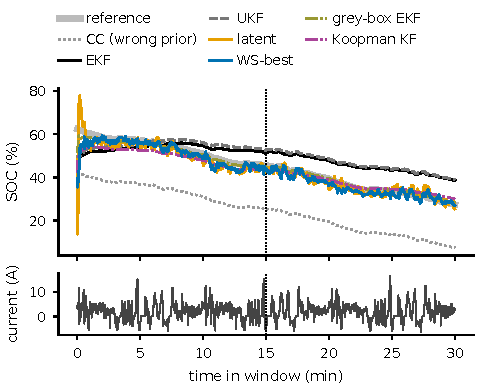
\includegraphics[width=0.49\textwidth]{us06_window.pdf}\hfill
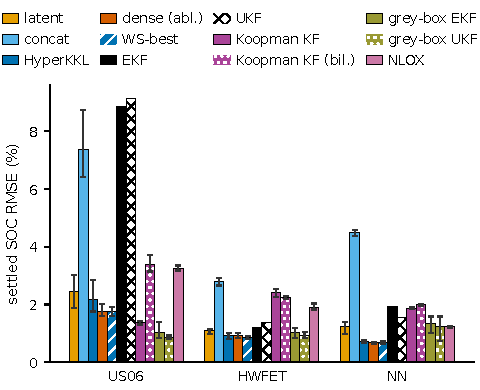
\includegraphics[width=0.49\textwidth]{rmse_test25.pdf}
\caption{Real data, 25$^\circ$C. Left: one US06 window from a prior 20\% off (the EKF settles on a biased SOC; the learned observer corrects it from data with a visible ripple). Dotted line: start of the settled window ($t\ge15$\,min); the current is positive on discharge. Right: settled SOC RMSE per method and test cycle, prior SOC $\pm20\%$; learned observers: mean over 3 seeds, whiskers min--max (\texttt{experiments/real/figures/}).}
\label{fig:real}
\end{figure}

\paragraph{Whole discharges (secondary).} From full charge with prior SOC 0.8, RMSE over $t\ge15$\,min: US06 WS-best \RealWholeWsBestUSZeroSix\ vs EKF \RealWholeEkfUSZeroSix\ / UKF \RealWholeUkfUSZeroSix; HWFTa \RealWholeWsBestHWFTa\ vs \RealWholeEkfHWFTa\ / \RealWholeUkfHWFTa; HWFTb \RealWholeWsBestHWFTb\ vs \RealWholeEkfHWFTb\ / \RealWholeUkfHWFTb; NN \RealWholeWsBestNN\ vs \RealWholeEkfNN\ / \RealWholeUkfNN. With hours to converge the filters match the learned observers on the mild cycles; the advantage on those cycles is convergence speed from a wrong prior, and on the aggressive cycle it is accuracy.

\paragraph{Temperature shift (secondary, 0$^\circ$C).} Models trained and identified at 25$^\circ$C only, evaluated on every 0$^\circ$C drive cycle. The claim does \emph{not} transfer: the EKF (Arrhenius-scaled resistances) is better on \RealZeroEkfBetter\ of \RealZeroNCycles\ cycles (learned \RealZeroWsRmseMin--\RealZeroWsRmseMax\,\%, EKF \RealZeroEkfRmseMin--\RealZeroEkfRmseMax\,\%); the learned observers win only on \RealZeroWsBetterCycles. The decoder has never seen the 0$^\circ$C voltage--SOC--current relationship, whereas the filter carries an explicit temperature model. Weight-space vs latent is decided for neither side on \RealZeroWsLatentTies\ of \RealZeroNCycles\ cycles. Training on several temperatures (the dataset covers $-20$ to 25$^\circ$C) is the obvious next step and was not part of the pre-registration.

\paragraph{Limitations (as recorded in the experiment report).} (1) The reference SOC is coulomb counting, the standard in this literature but itself an estimate (tester current error; capacity measured once at C/20 after the drive cycles, i.e.\ after some ageing; SOC $=1$ at the end of each CC--CV charge by definition); using the nominal 2.9\,Ah instead would shift the reference by up to 2.8\% SOC at the end of a discharge; the learned methods are trained on this reference and can absorb its convention. (2) One cell, one test campaign: windows within a cycle are dependent (handled by the block bootstrap), cell-to-cell variation is not sampled, and US06 has only \RealNwinUsZeroSix\ windows. (3) The advantage holds at the training temperature only. (4) The filters use a constant-parameter 2-RC circuit without hysteresis or SOC-dependent resistance, i.e.\ what a quick least-squares identification gives; a richer model (lookup tables from the HPPC tests, a hysteresis state) would narrow the gap and was not built. This is the incomplete-model regime of C3 by design. (5) The short-window protocol favours fast convergence. (6) The learned estimate has sample-level ripple. Deviations from the pre-registration (implementation only): filters run batched on GPU over the whole $Q,R$ grid (tested equal to individual filters); phase-1 simulations use clean outputs and no process noise; not run: the strict shape split, the residual alarm, NLOX, and the same-data baselines (\RealSameDataBaselines).
